\chapter{Soluzioni di viscosità}
In questa sezione richiamiamo alcune nozioni base sulle soluzioni viscose di equazioni alle derivate parziali (PDE) del secondo ordine e della loro variante parbolica. Senza addentrarci nell'analisi dettagliata di teoremi e preposizioni per il cui approfondimento \cite[vedi][]{fed:drag,giga:main,crand:lion,yun:giga}.
%%%%%%%%%%%%%%%%%%%%%%%%%%%%%%%%%%%%%%%%%%%%%%%%%%%%%%%%%%%%%%%%%%%%%%%%%%
%
%                            Section 2.1
%
%
%%%%%%%%%%%%%%%%%%%%%%%%%%%%%%%%%%%%%%%%%%%%%%%%%%%%%%%%%%%%%%%%%%%%%%%%%%
\section{Le soluzioni classiche non bastano}
Iniziamo subito con un esempio.
\begin{esempio}[\emph{Equazione eiconale}]
Consideriamo l'equazione
\begin{equation}
\label{eq:cp2-01}
|u'(x)| = 1,\text{ con $x\in(-1,1)$},
\end{equation}
questo è un caso particolare dell'equazione \emph{eiconale}
\[
|Du| = f(x).
\]
Supponiamo che esista una soluzione classica con condizioni di Dirichlet nulle, cioè $\exists\, u\in C^1(-1,1)$ che risolve \eqref{eq:cp2-01} con $u(-1)=u(1)=0$. Quindi per il noto teorema del valor medio esiste un punto $\xi\in (-1,1)$ tale che $u'(\xi)=0$, cioè $u$ non può risolvere \eqref{eq:cp2-01}. Inoltre, poichè $u\in C^1$ esiste un intervallo non vuoto $(-a,a)$ (con $0<a<1$) tale che $|u'(x)|<1$ per $x\in(-a,a)\subset(-1,1)$, quindi la \eqref{eq:cp2-01} viene contradetta in un intero intervallo.
\end{esempio}
Da qui la necessità di una nozione più debole di soluzione. Pensando all'esempio precedente, una prima idea sarebbe di richiedere che l'equazione sia soddisfatta solo nei punti dove la derivata esiste, questo ci porta ad una definizione di soluzione quasi ovunque. Tuttavia, usando sempre l'equazione eiconale, possiamo vedere come questa nozione sia buona per l'esistenza ma pessima per l'unicità.
\begin{esempio}[\emph{Funzioni di Rademacher}]
Le funzioni $u(x)=-|x|+1$ e $v(x)=|x|-1$ sono due differenti soluzioni quasi ovunque di \eqref{eq:cp2-01} che si annullano al bordo. Più in generale, le funzioni di Readmacher(vedi figura \ref{fig:cp2-01}) ci danno infinite soluzioni quasi ovunque per \eqref{eq:cp2-01}.
Queste sono cosi definite, per ogni $k\in \mathbb{N}$ e $i=0,1,\dots,2^{k-1}$
\[
u_k(x)=
\begin{cases}
  x+1-\frac{i}{2^{k-1}},\text{ se }x\in\left[-1+\frac{i}{2^{k-1}},-1+\frac{2i+1}{2^k}\right) \\
  -x-1 +\frac{i+1}{2^{k-1}},\text{ se }x\in\left[-1+\frac{2i+1}{2^k},-1+\frac{i+1}{2^{k-1}}\right)
\end{cases}
\]
\end{esempio}
\begin{figure}[!htb]
  \begin{center}
    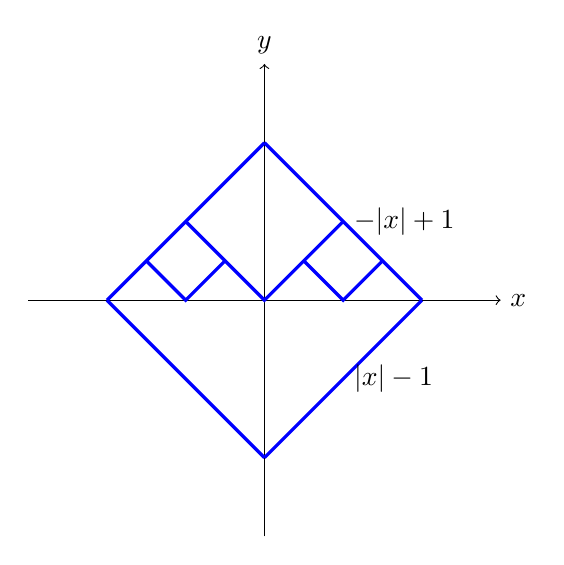
\begin{tikzpicture}[scale=2]

% Axis
      \draw[->] (-1.5,0.0) -- (1.5,0.0) node[anchor=west] {$x$};
      \draw[->] (0.0,-1.5) -- (0.0,1.5) node[anchor=south] {$y$};
% Radmacher Functions
    %k=0
      \begin{scope}[draw=blue,line width=1.2pt]
        \draw (-1.0,0.0) -- (0.0,1.0);
        \draw (0.0,1.0)  -- (0.5,0.5) node[anchor=west] {$-|x|+1$} -- (1.0,0.0);

        \draw (-1.0,0.0)  -- (0.0,-1.0);
        \draw (0.0,-1.0)  -- (0.5,-0.5) node[anchor=west] {$|x|-1$} -- (1.0,0.0);
%k=1
        \draw (-0.5,0.5) -- (-0.0,0.0) -- (0.5,0.5);
%k=2
        \draw (-0.75,0.25) -- (-0.5,0.0) -- (-0.25,0.25);
        \draw (0.25,0.25) -- (0.5,0.0) -- (0.75,0.25);
      \end{scope}

    \end{tikzpicture}
  \end{center}
  \caption{Funzioni di \emph{Readmacher}. Soluzioni quasi ovunque dell'equazione einoidale.}
  \label{fig:cp2-01}
\end{figure}

Nel 1982 Crandal and lions introdussero una differente nozione di soluzione debole (soluzioni viscose \cite[vedi][]{crand:lion}) che si comporta bene per molti PDE del primo e del secondo ordine, soddisfacendo proprietà di esistenza, unicità e stabiltà. 
%%%%%%%%%%%%%%%%%%%%%%%%%%%%%%%%%%%%%%%%%%%%%%%%%%%%%%%%%%%%%%%%%%%%%%%%%%
%
%                            Section 2.2
%
%
%%%%%%%%%%%%%%%%%%%%%%%%%%%%%%%%%%%%%%%%%%%%%%%%%%%%%%%%%%%%%%%%%%%%%%%%%%
\section{Nozione di soluzioni viscose}
Inziamo col introdurre la definizione di soluzione viscosa per PDE del secondo ordine, cioè equazioni del tipo
\begin{equation}
\label{eq:cp2-02}
F(x,u,Du,D^2u) = 0\text{ con }F:\mathbb{R}^N\times\mathbb{R}\times\mathbb{R}^N\times S(N)\to \mathbb{R},
\end{equation}
con $S(N)$ insieme delle matrici simmetriche $N\times N$, $u$ una funzione a volori reali definita in un sottoinsieme $\mathcal{O}$ di $\mathbb{R}^N$ e $Du$,$D^2u$ corrispondono al gradiente ed alla matrice delle derivate seconde di $u$. Al fine di applicare la teoria a un equazione del tipo \eqref{eq:cp2-02} (\cite[vedi][2]{crand:lion}), richiederemo che $F$ soddisfi le seguenti propietà
\begin{gather}
\label{eq:cp2-03}
F(x,r,p,X) \leq F(x,s,p,X) \quad \forall\,r\leq s,\\
\label{eq:cp2-04}
F(x,r,p,X) \leq F(x,r,p,Y) \quad \forall\,Y\leq X,
\end{gather}
con $r,s\in \mathbb{R},X,Y\in S(N)$ and $S(N)$ equipaggiato del solito ordine tra matrici. Se $F$ soddisfa \eqref{eq:cp2-03} allora si dirà \emph{ellitticamente degenere}, mentre se soddisfa \eqref{eq:cp2-04} si dirà \emph{propria}.
